\subsection{Zbiór "Diabetes"}
  \begin{figure}[H]
    \center
    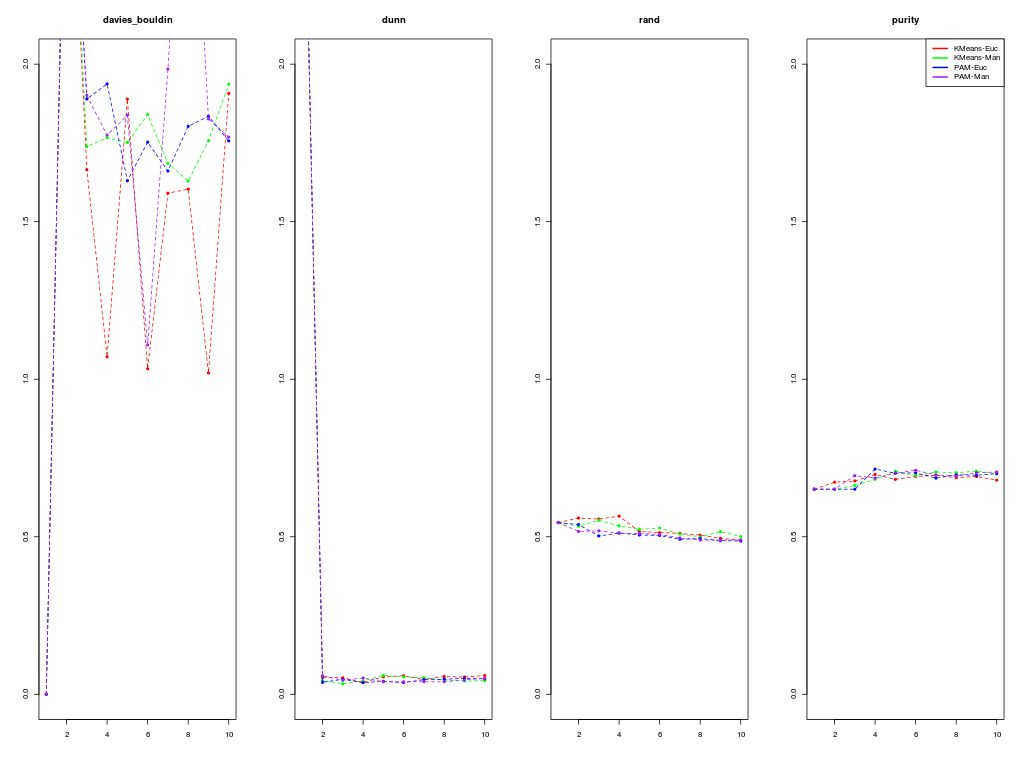
\includegraphics[width=\textwidth]{resources/plots/diabetes_metrics.png}
    \caption{Wykresy wartości metryk dla zbioru "Diabetes".}
  \end{figure}

  % latex table generated in R 3.4.4 by xtable 1.8-2 package
% Sun May  6 16:29:09 2018
\begin{table}[ht]
\centering
\begin{tabular}{llrlrr}
  \hline
alg & nb\_clus & davies\_bouldin & dunn & rand & purity \\ 
  \hline
KMeans-Euc & 1 & 0.00 & INF & 0.55 & 0.65 \\ 
  KMeans-Euc & 2 & 2.01 & 0.053 & 0.56 & 0.67 \\ 
  KMeans-Euc & 3 & 1.67 & 0.052 & 0.56 & 0.68 \\ 
  KMeans-Euc & 4 & 1.07 & 0.038 & 0.57 & 0.70 \\ 
  KMeans-Euc & 5 & 1.89 & 0.056 & 0.52 & 0.68 \\ 
  KMeans-Euc & 6 & 1.03 & 0.059 & 0.51 & 0.69 \\ 
  KMeans-Euc & 7 & 1.59 & 0.048 & 0.51 & 0.69 \\ 
  KMeans-Euc & 8 & 1.60 & 0.056 & 0.51 & 0.69 \\ 
  KMeans-Euc & 9 & 1.02 & 0.055 & 0.49 & 0.69 \\ 
  KMeans-Euc & 10 & 1.91 & 0.06 & 0.49 & 0.68 \\ 
  KMeans-Man & 1 & 0.00 & INF & 0.55 & 0.65 \\ 
  KMeans-Man & 2 & 2.16 & 0.043 & 0.53 & 0.65 \\ 
  KMeans-Man & 3 & 1.74 & 0.034 & 0.55 & 0.66 \\ 
  KMeans-Man & 4 & 1.77 & 0.043 & 0.54 & 0.68 \\ 
  KMeans-Man & 5 & 1.75 & 0.06 & 0.52 & 0.71 \\ 
  KMeans-Man & 6 & 1.84 & 0.056 & 0.53 & 0.69 \\ 
  KMeans-Man & 7 & 1.69 & 0.052 & 0.51 & 0.71 \\ 
  KMeans-Man & 8 & 1.63 & 0.046 & 0.50 & 0.70 \\ 
  KMeans-Man & 9 & 1.76 & 0.042 & 0.52 & 0.71 \\ 
  KMeans-Man & 10 & 1.94 & 0.043 & 0.50 & 0.70 \\ 
  PAM-Euc & 1 & 0.00 & INF & 0.55 & 0.65 \\ 
  PAM-Euc & 2 & 2.19 & 0.038 & 0.54 & 0.65 \\ 
  PAM-Euc & 3 & 1.89 & 0.048 & 0.50 & 0.65 \\ 
  PAM-Euc & 4 & 1.94 & 0.037 & 0.51 & 0.71 \\ 
  PAM-Euc & 5 & 1.63 & 0.041 & 0.51 & 0.70 \\ 
  PAM-Euc & 6 & 1.75 & 0.037 & 0.50 & 0.70 \\ 
  PAM-Euc & 7 & 1.66 & 0.047 & 0.49 & 0.69 \\ 
  PAM-Euc & 8 & 1.80 & 0.048 & 0.49 & 0.70 \\ 
  PAM-Euc & 9 & 1.83 & 0.051 & 0.49 & 0.69 \\ 
  PAM-Euc & 10 & 1.76 & 0.049 & 0.49 & 0.70 \\ 
  PAM-Man & 1 & 0.00 & INF & 0.55 & 0.65 \\ 
  PAM-Man & 2 & 2.35 & 0.058 & 0.52 & 0.65 \\ 
  PAM-Man & 3 & 1.90 & 0.045 & 0.52 & 0.69 \\ 
  PAM-Man & 4 & 1.77 & 0.052 & 0.51 & 0.69 \\ 
  PAM-Man & 5 & 1.84 & 0.04 & 0.51 & 0.70 \\ 
  PAM-Man & 6 & 1.11 & 0.04 & 0.51 & 0.71 \\ 
  PAM-Man & 7 & 1.98 & 0.04 & 0.50 & 0.70 \\ 
  PAM-Man & 8 & 2.02 & 0.04 & 0.49 & 0.69 \\ 
  PAM-Man & 9 & 1.83 & 0.046 & 0.49 & 0.70 \\ 
  PAM-Man & 10 & 1.77 & 0.051 & 0.49 & 0.71 \\ 
   \hline
\end{tabular}
\end{table}


  \subsubsection{Algorytm K-Means (Euclidean)} 
    \begin{figure}[H]
      \center
      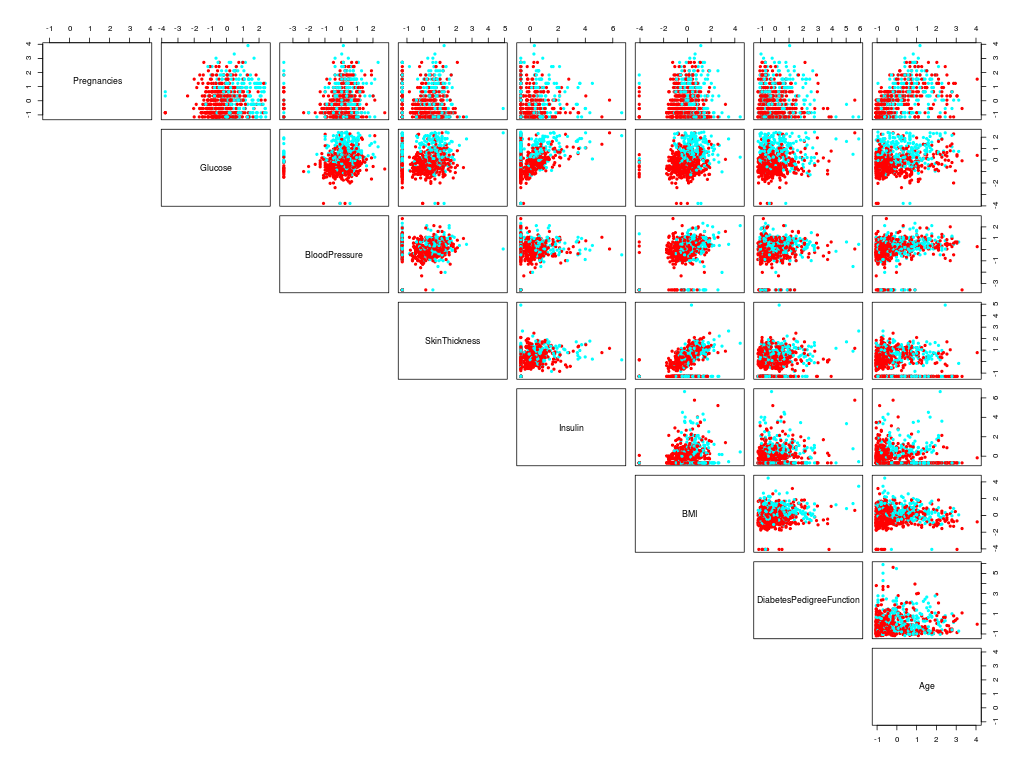
\includegraphics[width=0.8\textwidth]{resources/plots/diabetes_KMeans-Euc_scatter.png}
      \caption{Wynik klasteryzacji dla algorytmu KMeans (Euclidean) dla zbioru "Diabetes".}
    \end{figure}
    \begin{figure}[H]
      \center
      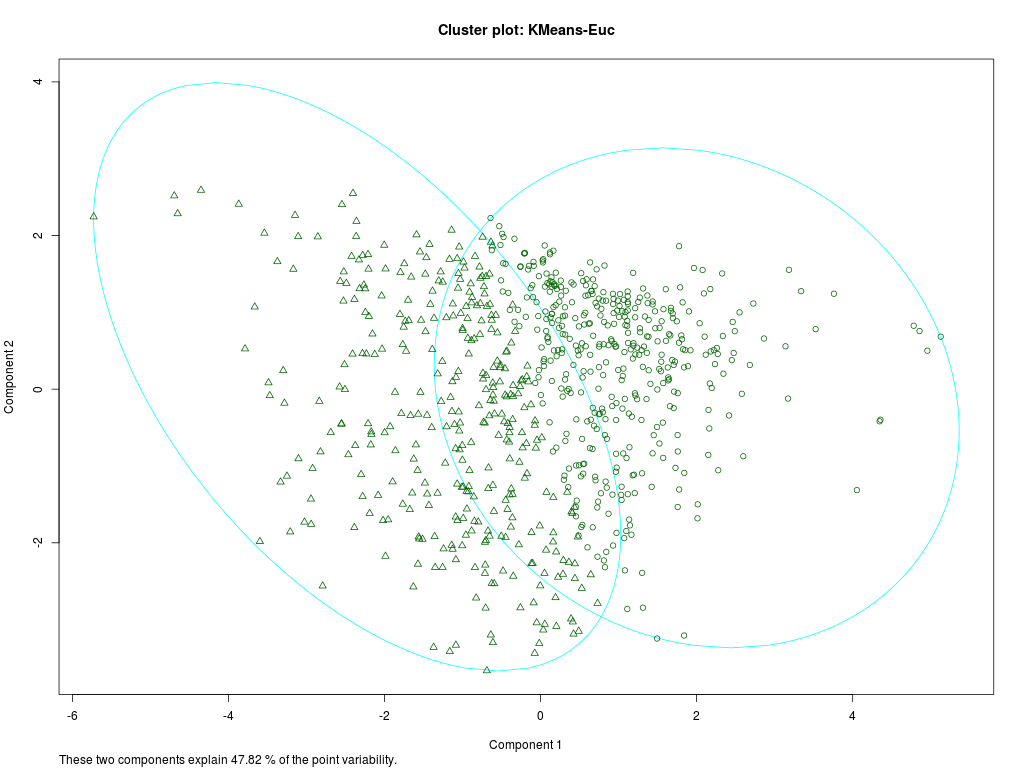
\includegraphics[width=0.8\textwidth]{resources/plots/diabetes_KMeans-Euc_cluster.png}
      \caption{Klastry dla algorytmu KMeans (Euclidean) dla zbioru "Diabetes".}
    \end{figure}

  \subsubsection{Algorytm K-Means (Manhattan)} 
    \begin{figure}[H]
      \center
      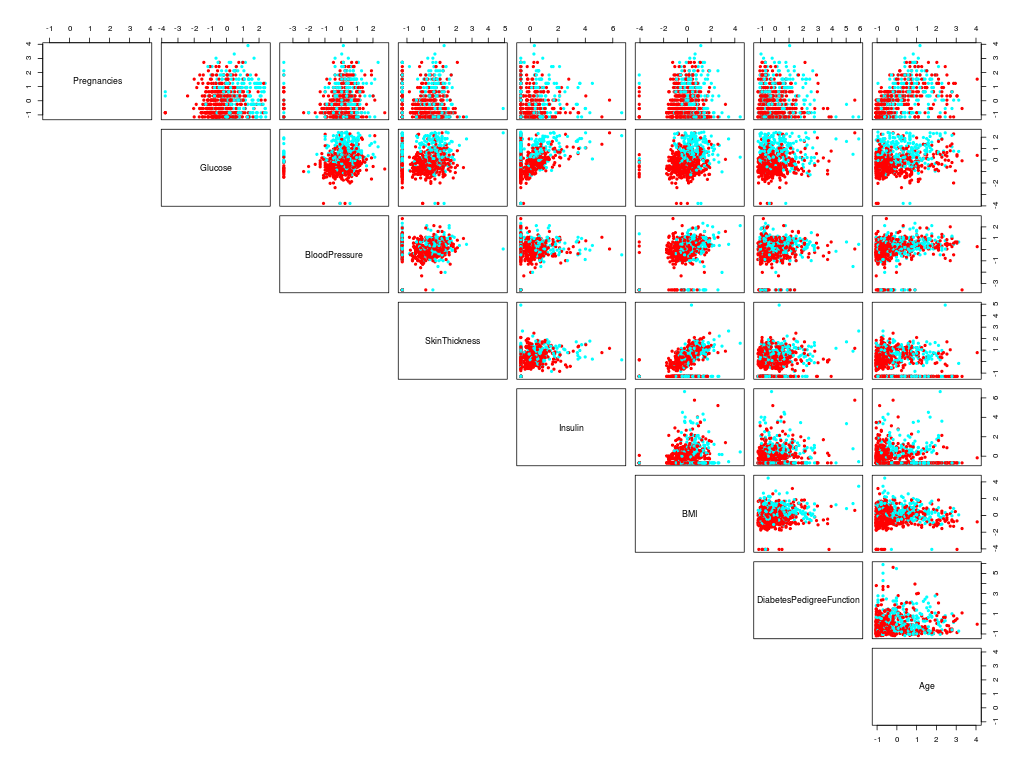
\includegraphics[width=0.8\textwidth]{resources/plots/diabetes_KMeans-Man_scatter.png}
      \caption{Wynik klasteryzacji dla algorytmu KMeans (Manhattan) dla zbioru "Diabetes".}
    \end{figure}
    \begin{figure}[H]
      \center
      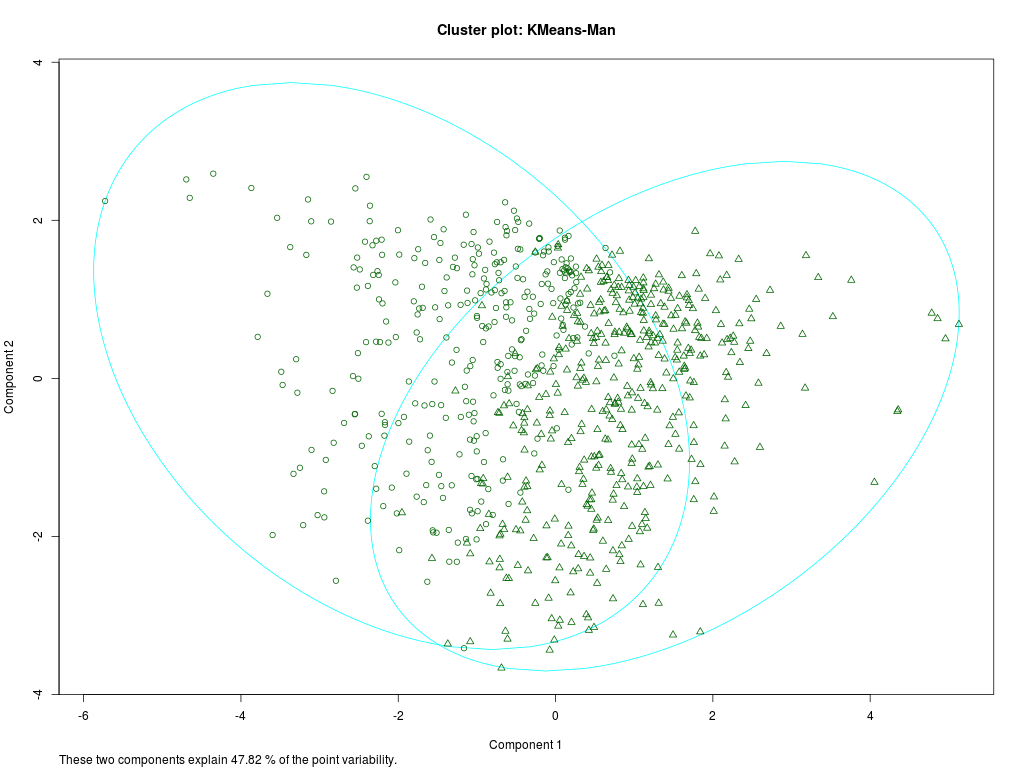
\includegraphics[width=0.8\textwidth]{resources/plots/diabetes_KMeans-Man_cluster.png}
      \caption{Klastry dla algorytmu KMeans (Manhattan) dla zbioru "Diabetes".}
    \end{figure}

  \subsubsection{Algorytm PAM (Euclidean)} 
    \begin{figure}[H]
      \center
      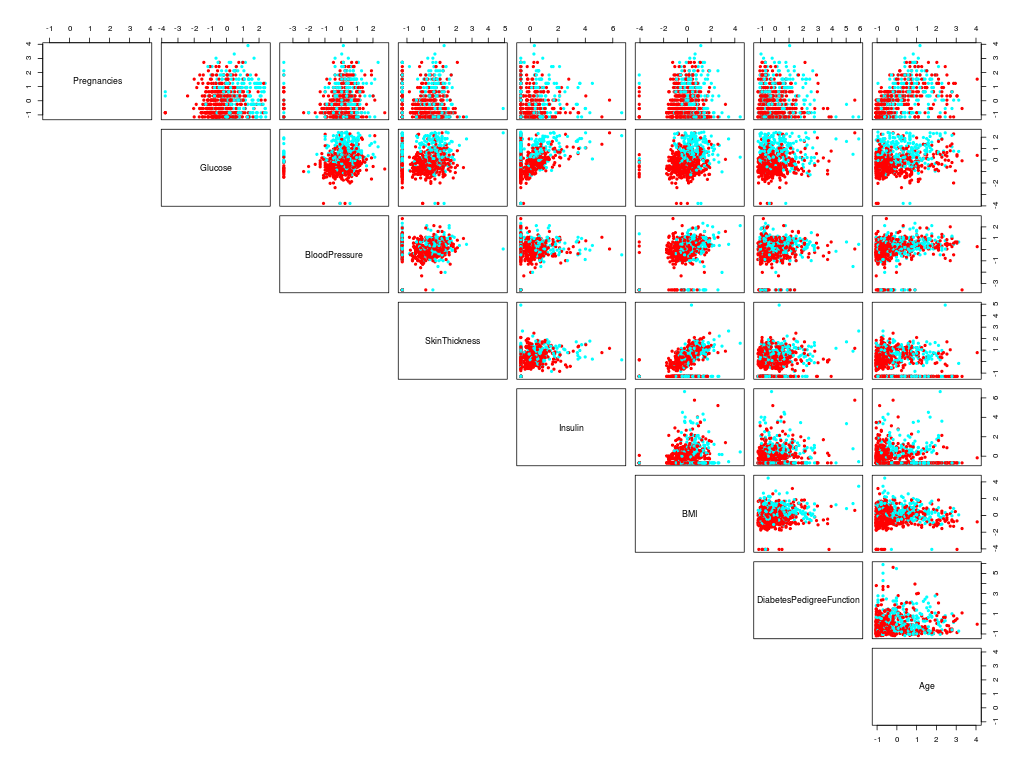
\includegraphics[width=0.8\textwidth]{resources/plots/diabetes_PAM-Euc_scatter.png}
      \caption{Wynik klasteryzacji dla algorytmu PAM (Euclidean) dla zbioru "Diabetes".}
    \end{figure}
    \begin{figure}[H]
      \center
      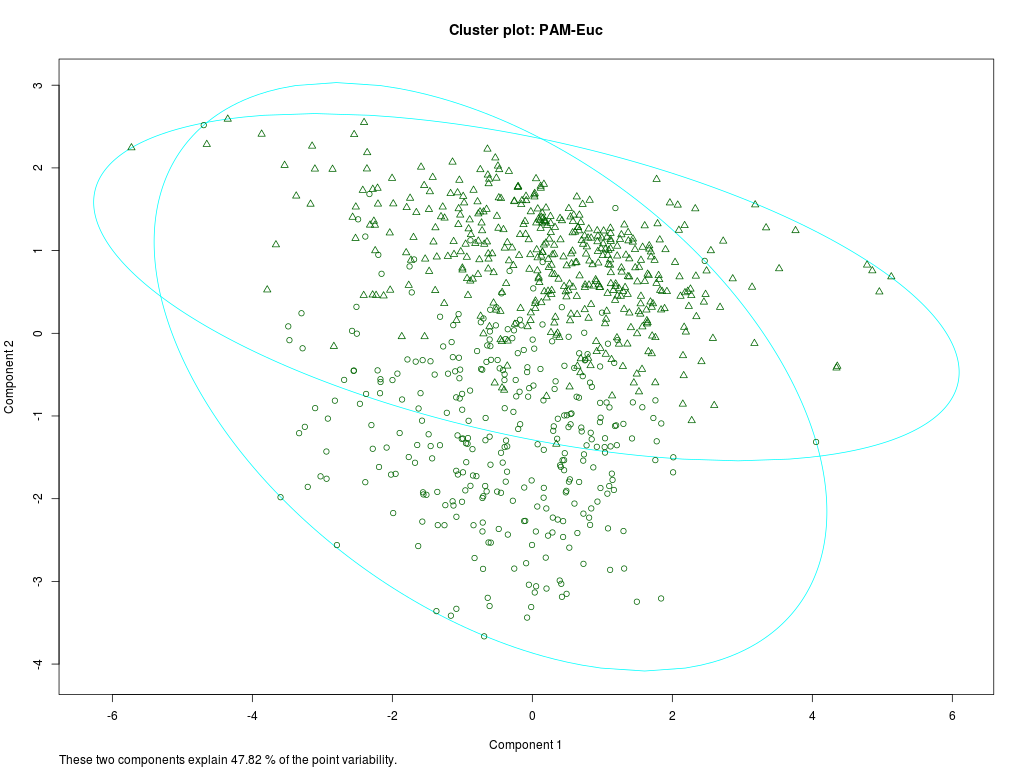
\includegraphics[width=0.8\textwidth]{resources/plots/diabetes_PAM-Euc_cluster.png}
      \caption{Klastry dla algorytmu PAM (Euclidean) dla zbioru "Diabetes".}
    \end{figure}

  \subsubsection{Algorytm PAM (Manhattan)} 
    \begin{figure}[H]
      \center
      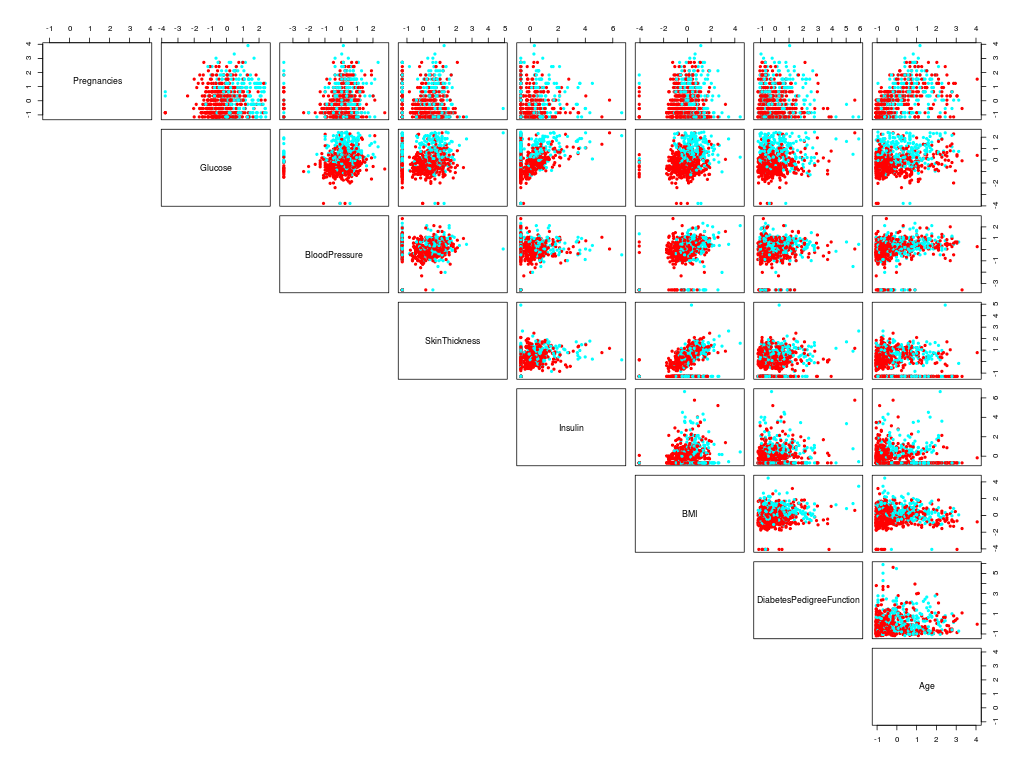
\includegraphics[width=0.8\textwidth]{resources/plots/diabetes_PAM-Man_scatter.png}
      \caption{Wynik klasteryzacji dla algorytmu PAM (Manhattan) dla zbioru "Diabetes".}
    \end{figure}
    \begin{figure}[H]
      \center
      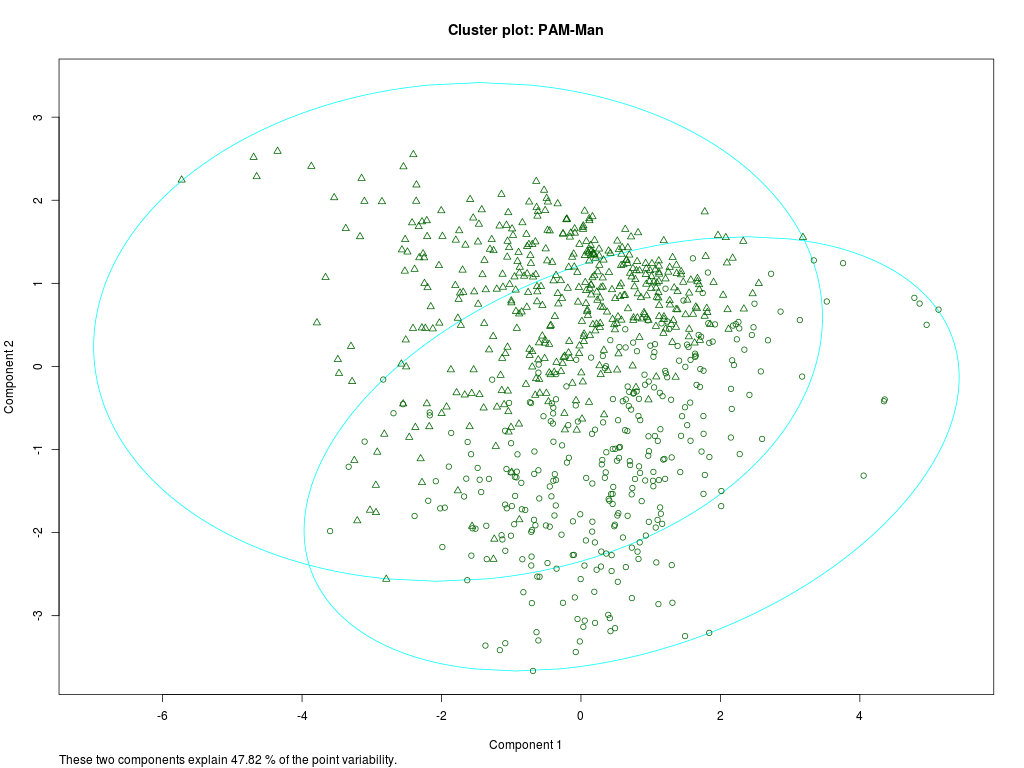
\includegraphics[width=0.8\textwidth]{resources/plots/diabetes_PAM-Man_cluster.png}
      \caption{Klastry dla algorytmu PAM (Manhattan) dla zbioru "Diabetes".}
    \end{figure}
